\documentclass{article}[12pt]
\usepackage{geometry}
\usepackage{graphicx}

\geometry{margin=1.2in}
\linespread{1.1}
\setlength{\parskip}{1em}
\setlength{\parindent}{0in}
\setlength{\abovecaptionskip}{0in}
\setlength{\belowcaptionskip}{1em}

\graphicspath{ {.} }

\begin{document}

{\huge \textbf{Part C}}

\begin{enumerate}
    \item \textbf{Pinging from h1 to h5}

    \begin{figure}[!h]
        \centering
        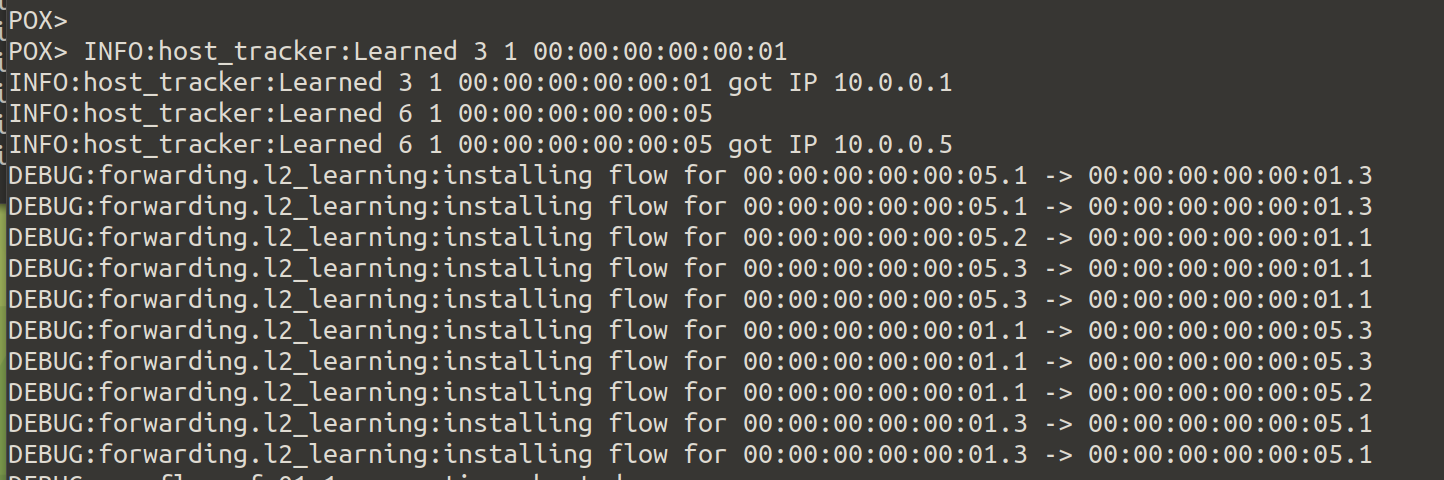
\includegraphics[width=\textwidth,height=\textheight,keepaspectratio]{ping.png}
    \end{figure}

    To get from h1 to h5, the packet must pass through s3, s2, s1, s5, and finally s6.

    The controller installs the correct flow rules needed so that packets can pass from h1 to h5 along this path.

    We first see the controller getting the IP addresses for the two hosts we are pinging and the respective MAC addrs of the switches they are attached to. Then the controller begins to install flows that allow forwarding along the s3 => s2 => s1 => s5 => s6 path.

    The l2\_learning logs only show the MAC addresses being matched to and the in / out ports to use if the packet matches. We see 5 entries for the MAC of h1, and 5 entries for the MAC of h5. Each entry is adding a flow rule setting the output port if it matches to the input port and src/dst MACs. 

    \item \textbf{RTT for first 5 pings}
    
    \begin{figure}[!h]
        \centering
        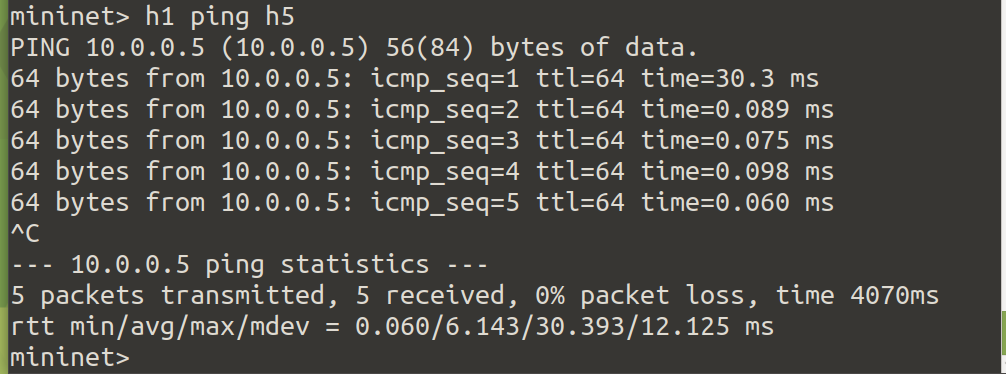
\includegraphics[width=\textwidth,height=\textheight,keepaspectratio]{rtt.png}
    \end{figure}

    The first ping is significantly slower because it needs to wait for the controller to install the flow rules.

    \item \textbf{Flow rules for all switches}
    
    Screenshots taken after pinging h1 to h5.

    Before the ping, all the flow tables started off with two entries which pointed to the controller. After the ping, we can see entries in the tables of all the switches that the packet passed through. 
    
    After the ping, s4 and s7 still don't have any flow rules defined in them (besides the ones pointing to the controller). This is because the packets going from h1 to h5 did not need to pass through these switches, so they were left out of the communication.

    The collective effect of these flows is destination-based forwarding, since it's allowing any and all traffic to flow between h1 and h5 without specific matches being required. It differs from partA and partB because there we restricted our forwarding to specific matches at the IP and MAC levels.
    
    \begin{figure}[!h]
        \centering
        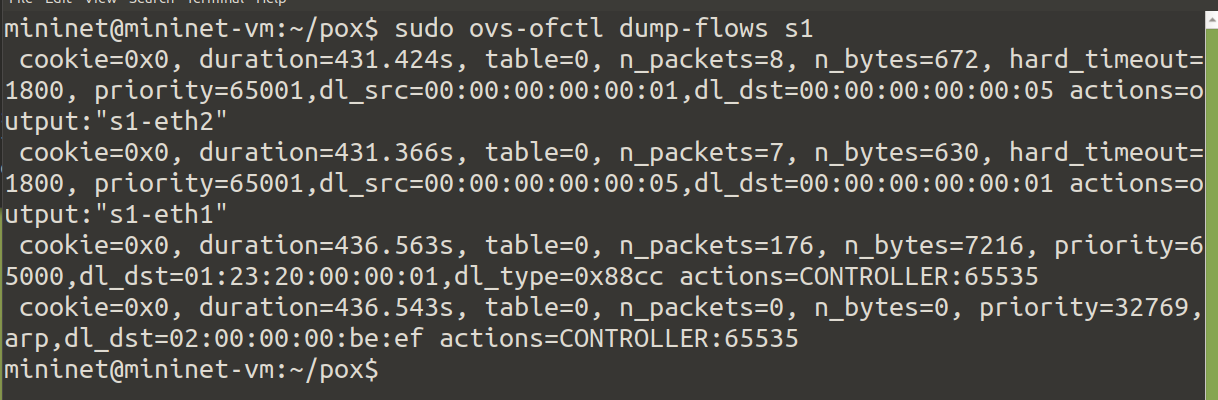
\includegraphics[width=\textwidth,height=\textheight,keepaspectratio]{s1.png}
        \caption{s1}
    \end{figure}

    \begin{figure}[!h]
        \centering
        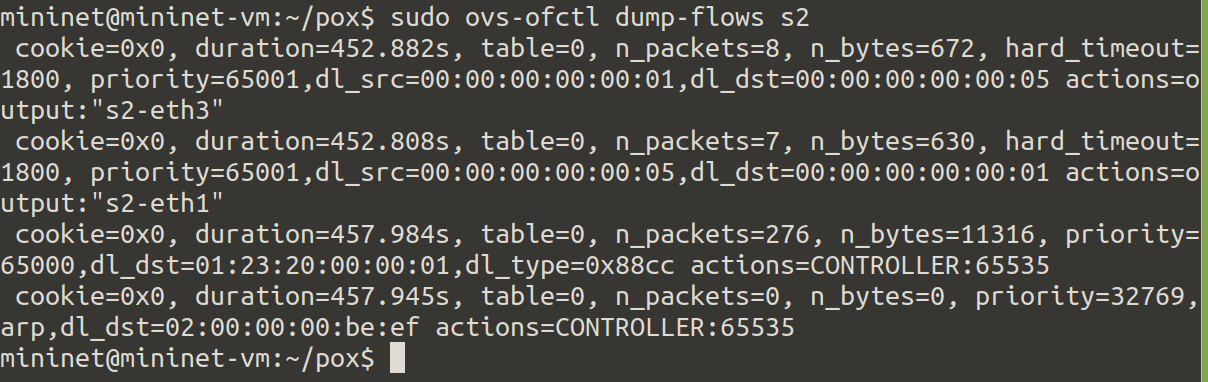
\includegraphics[width=\textwidth,height=\textheight,keepaspectratio]{s2.png}
        \caption{s2}
    \end{figure}

    \begin{figure}[!h]
        \centering
        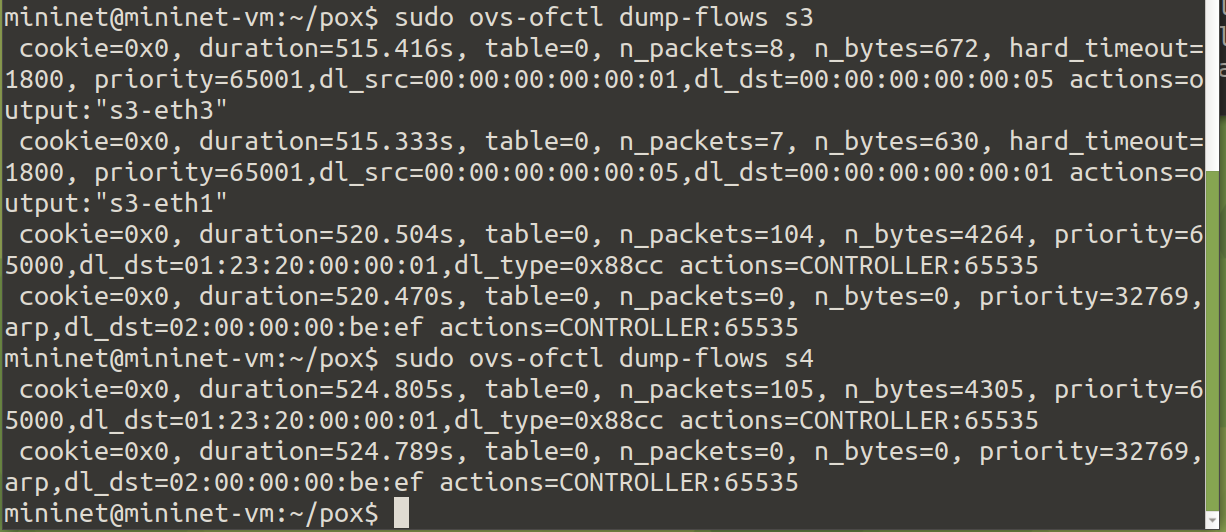
\includegraphics[width=\textwidth,height=\textheight,keepaspectratio]{s3s4.png}
        \caption{s3 and s4}
    \end{figure}

    \begin{figure}[!h]
        \centering
        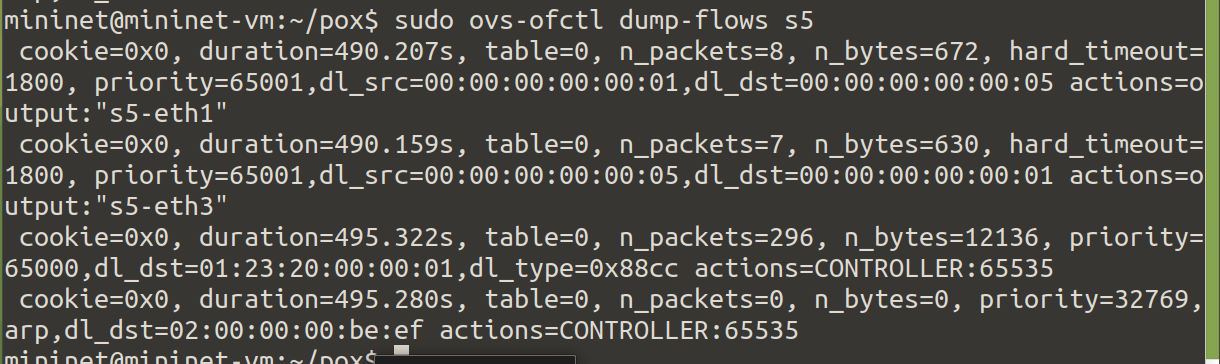
\includegraphics[width=\textwidth,height=\textheight,keepaspectratio]{s5.png}
        \caption{s5}
    \end{figure}

    \begin{figure}[!h]
        \centering
        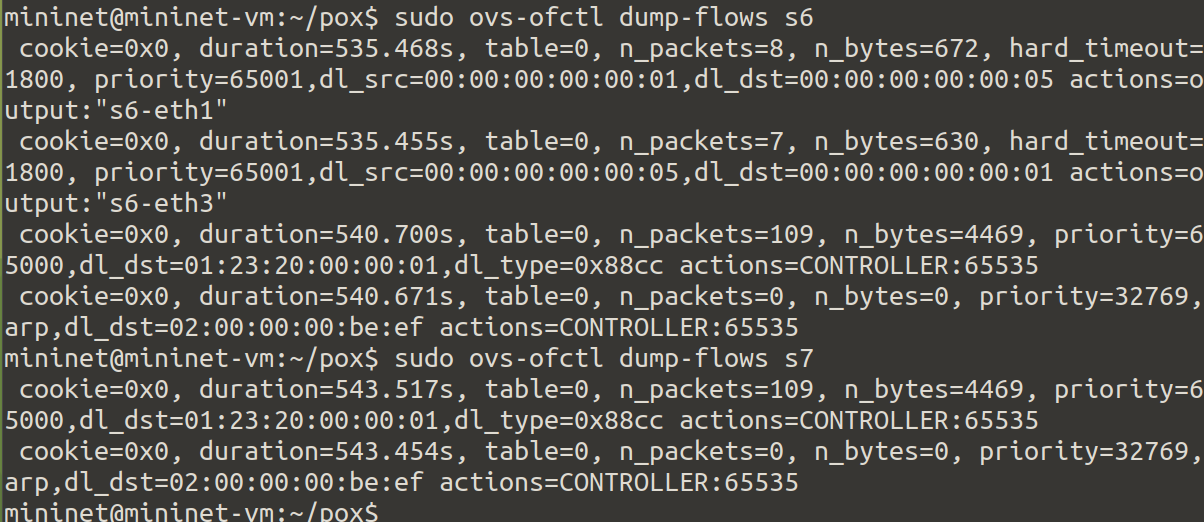
\includegraphics[width=\textwidth,height=\textheight,keepaspectratio]{s6s7.png}
        \caption{s6 and s7}
    \end{figure}
    
\end{enumerate}

\end{document}